\PassOptionsToPackage{table}{xcolor}
\documentclass[10pt]{beamer}
\usepackage[english]{babel}

\usetheme{metropolis}
\usepackage{smartdiagram}
\usepackage{listings}
\usepackage{booktabs}
\usepackage[scale=2]{ccicons}%creative commons
\setbeamercovered{transparent}%invisible by default
\usepackage{array}
\newcolumntype{L}[1]{>{\raggedright\let\newline\\\arraybackslash\hspace{0pt}}m{#1}}
\newcolumntype{C}[1]{>{\centering\let\newline\\\arraybackslash\hspace{0pt}}m{#1}}
\newcolumntype{R}[1]{>{\raggedleft\let\newline\\\arraybackslash\hspace{0pt}}m{#1}}

\usepackage{pgfplots}
\usepgfplotslibrary{dateplot}
\usepackage{tikz}
\usetikzlibrary{positioning,chains,fit,shapes,calc,automata,positioning}
\newcommand{\mycomment}[1]{}
\usepackage{fancyvrb}
\usepackage{ifpdf}                        % To check if pdflatex is used.

\ifpdf
  \DeclareGraphicsRule{*}{mps}{*}{}       % To include metapost files.
\fi
% *****************************************************************************
% Matematica 
% *****************************************************************************

%\usepackage{amssymb}
%\usepackage{mathtools}                    % Add support for cramped,
					  
%\usepackage[euler]{flexisym}
%\usepackage{breqn}                        % Breqn
%\makeatletter
%   \def\eqnumsize{\normalfont \Tf@font}      % Add support to Minion Pro
%\makeatother
%\setkeys{breqn}{labelprefix={eq:}}


%\usepackage{asymptote}
%\usepackage[loop, controls]{animate}

\graphicspath{{./}, {./Images/}}

\lstdefinelanguage{Kotlin}{
  keywords={package, as, typealias, this, super, val, var, fun, for, null, true, false, is, in, throw, return, break, continue, object, if, try, else, while, do, when, yield, typeof, yield, typeof, class, interface, enum, object, override, public, private, get, set, import, abstract, },
  keywordstyle=\color{blue}\bfseries,
  ndkeywords={@Deprecated, Int, Integer, Float, Double, String, Runnable, dynamic},
  ndkeywordstyle=\color{red}\bfseries,
  emph={println, return@, forEach,},
  emphstyle={\color{red}},
  identifierstyle=\color{black},
  sensitive=true,
  commentstyle=\color{gray}\ttfamily,
  comment=[l]{//},
  morecomment=[s]{/*}{*/},
  stringstyle=\color{gray}\ttfamily,
  morestring=[b]",
  morestring=[s]{"""*}{*"""},
}

\providecommand{\ie}{i.\,e.}
\providecommand{\Ie}{I.\,e.}
\providecommand{\eg}{e.\,g.}
\providecommand{\Eg}{E.\,g.} 

\metroset{block=fill}
\metroset{titleformat frame=smallcaps}

\title{Scala cruise} 
\subtitle{Snorkelling in some of the Scala features}
% crash course in Scala
\date{\today}
\author[A. Candolini]{Alessandro Candolini}
%\institute{Department of Physics, University of Trieste}
% \titlegraphic{\hfill\includegraphics[height=1.5cm]{logo/logo}}

\begin{document}

\maketitle

\begin{frame}{Itinerary}
  \setbeamertemplate{section in toc}[sections numbered]
  \tableofcontents[hideallsubsections]
\end{frame}

\section{Let's meet Scala}

\begin{frame}
\begin{figure}
\centering
\includegraphics[height=.6\textheight]{martin}
\caption{Martin Odersky, the creator of Scala}
\end{figure}
\end{frame}

% Odersky viewpoint influences the look and feel and development of the Scala lang => synergy between OOP and FP 

\begin{frame}[fragile]
Scala programming language is:
\begin{itemize}
\item general purpose 
\item strongly statically typed (with type inference) 
\item compiling primarily to JVM 8+ bytecode%
\footnote{\texttt{scala.js} compiles to JS; \texttt{scala native} targets LLVM; jdk 9+ compatibility might require support; there is a Scala REPL.}
\item interoperable with Java 8+
\end{itemize}
\end{frame}

\begin{frame}
Scala supports 
\begin{itemize}
\item OOP
\item FP 
\end{itemize}
\end{frame}

\begin{frame}[fragile]
\begin{lstlisting}[language=Scala, basicstyle=\ttfamily]
val value : Int  = 2;
val text : String = "hello";
\end{lstlisting}
\end{frame}

\begin{frame}[fragile]
\begin{lstlisting}[language=Scala, basicstyle=\ttfamily]
val value : Int  = 2
val text : String = "hello" 
\end{lstlisting}
\end{frame}

\begin{frame}[fragile]
\begin{lstlisting}[language=Scala, basicstyle=\ttfamily]
val value = 2
val text = "hello" 
\end{lstlisting}
\end{frame}

\begin{frame}[fragile]
\begin{lstlisting}[language=Scala, basicstyle=\ttfamily]
val value = 2
val text = "hello"

print(text)
print(s"$value-$text") // string interpolation 
print(s"${value*2}")
\end{lstlisting}
\end{frame}

\begin{frame}[fragile]
\begin{lstlisting}[language=Scala, basicstyle=\ttfamily]
var value = 2
val text = "hello" 

value = 4
text = "hello" // !!! forbidden 
\end{lstlisting}
\end{frame}

\begin{frame}[fragile]
\begin{lstlisting}[language=Scala, basicstyle=\ttfamily]
def square(x : Int) : Int = {
  return x*x
}
\end{lstlisting}
\end{frame}

\begin{frame}[fragile]
\begin{lstlisting}[language=Scala, basicstyle=\ttfamily]
def square(x : Int) = x*x
\end{lstlisting}
\end{frame}

\begin{frame}[fragile]
\begin{lstlisting}[language=Scala, basicstyle=\ttfamily]
def abs(x : Int) =
  if (x >= 0) // if statement 
    x 
  else 
    -x  
\end{lstlisting}
\end{frame}

\begin{frame}[fragile]
\begin{lstlisting}[language=Scala, basicstyle=\ttfamily]
def id(x : Int) : Int = {
  if (x >= 0) { // if control flow  (imperative) 
    print(s"$x")
  }
  x
}

id(-2)
id(2)
\end{lstlisting}
\end{frame}


\begin{frame}[fragile]
\begin{lstlisting}[language=Scala, basicstyle=\ttfamily]
def square(x : Int) = x*x

square(2+3+4) // <-- how is this evaluated?
\end{lstlisting}
\end{frame}

\mycomment{%

\begin{frame}[fragile]
\begin{lstlisting}[language=Scala, basicstyle=\ttfamily]
def log(message : String) = ???
\end{lstlisting}
\end{frame}

\begin{frame}[fragile]
\begin{lstlisting}[language=Scala, basicstyle=\ttfamily]
def log(message : String) : Unit = ???

// unit type
\end{lstlisting}
\end{frame}


\begin{frame}[fragile]
\begin{lstlisting}[language=Scala, basicstyle=\ttfamily]
class Logger {

  def log(message : String) = ???

}
\end{lstlisting}
\end{frame}


\begin{frame}[fragile]
\begin{lstlisting}[language=Scala, basicstyle=\ttfamily]
trait Logger {
  def log(message : String)
}

class PrintLogger extends Logger {
  override def log(message: String) = {
    print(message)
  }
}
class ProductionLogger() extends Logger {
  override def log(message: String) = {
  }
}
\end{lstlisting}
\end{frame}

\begin{frame}[fragile]
\begin{lstlisting}[language=Scala, basicstyle=\ttfamily]
val logger : Logger = ???
// ...
logger.log("hello")  
\end{lstlisting}
\end{frame}

\begin{frame}[fragile]
\begin{lstlisting}[language=Scala, basicstyle=\ttfamily]
val logger : Logger = ???
// ...
logger.log("hello" + sqrt(2-3+10))  
\end{lstlisting}
\end{frame}

\begin{frame}[fragile]
\begin{lstlisting}[language=Scala, basicstyle=\ttfamily]
trait Logger {
  def log(message : => String) 
 // call by name vs call by value 
}
\end{lstlisting}
\end{frame}

\begin{frame}[fragile]
\begin{lstlisting}[language=Scala, basicstyle=\ttfamily]
def squareCallByName(x : => Int) = x*x
\end{lstlisting}
\end{frame}


\begin{frame}[fragile]
\begin{lstlisting}[language=Scala, basicstyle=\ttfamily]
val function : Int => Int = square
\end{lstlisting}
\end{frame}

\begin{frame}[fragile]
\begin{lstlisting}[language=Scala, basicstyle=\ttfamily]
def f(x : Int, y : Int) : Int = x + y
def g(y : Int) : Int = f(1,y)
def h(y : Int) : Int => Int = f(_,y)

f(2,3)
g(3)
h(2)(3)
\end{lstlisting}
\end{frame}

}

\begin{frame}[fragile]
\begin{lstlisting}[language=Scala, basicstyle=\ttfamily]
def div(x : Double) : Double = 1/x

div(1) // 1 
div(2) // 0.5 
div(0) // java.lang.ArithmeticException: / by zero
\end{lstlisting}
\end{frame}


\begin{frame}[fragile]
\begin{lstlisting}[language=Scala, basicstyle=\ttfamily]
def div(x : Double) : Double = 
  if ( x != 0 ) 
     1/x 
  else 
     null // !!!
\end{lstlisting}
\end{frame}

\begin{frame}[fragile]
\begin{lstlisting}[language=Scala, basicstyle=\ttfamily]
def div(x : Double) : Option[Double] =
  if ( x != 0 ) 
     Some[Double](1/x) 
  else 
     None
\end{lstlisting}
\end{frame}
\begin{frame}[fragile]
\begin{lstlisting}[language=Scala, basicstyle=\ttfamily]
def div(x : Double) : Option[Double] =
  if ( x != 0 ) 
     Some(1/x) 
  else 
     None
\end{lstlisting}
\end{frame}
\begin{frame}[fragile]
\begin{lstlisting}[language=Scala, basicstyle=\ttfamily]
def div(x : Double) = 
  if ( x != 0 ) 
     Some(1/x) 
  else 
     None
\end{lstlisting}
\end{frame}

\begin{frame}[fragile]
\begin{lstlisting}[language=Scala, basicstyle=\ttfamily]
def square(x : Double) = x*x 

def div(x : Double) = 
  if ( x != 0 ) Some(1/x) else None

square(div(3)) // !! Type mismatch 

val twice = 2*div(3) // !! Type mismatch 
\end{lstlisting}
\end{frame}

\begin{frame}[fragile]
\begin{lstlisting}[language=Scala, basicstyle=\ttfamily]
def div(x : Double) = 
  if ( x != 0 ) Some(1/x) else None

val twice : Option[Double] 
   = div(3).map( value => 2*value)
\end{lstlisting}
\end{frame}

\begin{frame}[fragile]
\begin{lstlisting}[language=Scala, basicstyle=\ttfamily]
def div(x : Double) = 
  if ( x != 0 ) Some(1/x) else None

div(3).map(2*_)
\end{lstlisting}
\end{frame}

\begin{frame}[fragile]
\begin{lstlisting}[language=Scala, basicstyle=\ttfamily]
def square(x : Int) = x*x 

def div(x : Int) = 
  if ( x != 0 ) Some(1/x) else None

div(0).map(value => square(value))
div(0).map(square)
\end{lstlisting}
\end{frame}

\begin{frame}[fragile]
\begin{lstlisting}[language=Scala, basicstyle=\ttfamily]
def div(x : Double) = 
  if ( x != 0 ) Some(1/x) else None

def someFunction(x : Double) : Option[Double] = ???

div(0).flatMap(anotherFunction)
\end{lstlisting}
\end{frame}

\begin{frame}
Crash course in Monads 
\end{frame}

\begin{frame}[fragile]
\begin{quotation}
All told, a monad is just a monoid in the category of endofunctors 
\end{quotation}
\begin{flushright}
S. Mac Lane
\end{flushright}
\begin{quotation}
Monads are return types at guide you through the happy path 
\end{quotation}
\begin{flushright}
E. Mejier 
\end{flushright}
\begin{quotation}
Monads are like burritos 
\end{quotation}
\begin{flushright}
Brent Yorgey
\end{flushright}
\end{frame}

\begin{frame}[fragile]
\begin{lstlisting}[language=Scala, basicstyle=\ttfamily]
def f(a:A) : Future[B]
def g(b:B) : Future[C]

val a : A = ???

f(a).flatMap(g)
\end{lstlisting}
\end{frame}


\begin{frame}
\begin{itemize}
\item Option[Option[A]] $\rightarrow$ Option[A]
\item Future[Future[A]] $\rightarrow$ Future[A]
\item List[List[A]] $\rightarrow$ List[A]
\end{itemize}
\end{frame}
\begin{frame}[fragile]
Compare this to \emph{ad-hoc} Kotlin syntax for nullable types 
\begin{lstlisting}[language=Scala, basicstyle=\ttfamily]
var value : Int? = 0

value?.let { it }
\end{lstlisting}
\end{frame}

\begin{frame}[fragile]
\begin{lstlisting}[language=Scala, basicstyle=\ttfamily]
// value classes 
class ProductId(val id: Int) extends AnyVal 

// case classes 
case class ProductDetails(
  id: ProductId,
  description: String
) // notice: no val/var 
\end{lstlisting}
\end{frame}


\begin{frame}[fragile]
\begin{lstlisting}[language=Scala, basicstyle=\ttfamily]
def fetchIds() : Future[Seq[ProductId]] = ???

def fetchDetails(ids : Set[ProductId]) 
   : Future[Map[ProductId, ProductDetails] = ???

def hydrate() = 
   fetchIds().flatmap( ??? )

\end{lstlisting}
\end{frame}






%\begin{frame}[fragile]
%\begin{lstlisting}[language=Scala, basicstyle=\ttfamily]
%\end{lstlisting}
%\end{frame}

%\begin{frame}[fragile]
%\begin{lstlisting}[language=Scala, basicstyle=\ttfamily]
%\end{lstlisting}
%\end{frame}


%\begin{frame}[fragile]
%\begin{lstlisting}[language=Scala, basicstyle=\ttfamily]
%\end{lstlisting}
%\end{frame}










%\begin{frame}[fragile]
%\begin{lstlisting}[language=Scala, basicstyle=\ttfamily]
%\end{lstlisting}
%\end{frame}




% Error handling 
% Case classes
% Value classes
% Pattern matching 
% Option
% Future 
% implicits 



%\section{We live in a concurrent world}
%\begin{frame}[fragile]
%	% Spoiler
%	\begin{figure}
%		\centering
%		\includegraphics[width=.8\textwidth]{concurrency_coffee}
%		\caption{\url{https://joearms.github.io/published/2013-04-05-concurrent-and-parallel-programming.html}}
%	\end{figure}
%\end{frame}
%\begin{frame}[fragile]
%Is concurrency relevant for mobile development?
%	\begin{itemize} 
%		\item<2-> IO (\eg, network, etc) 
%		\item<3-> sensors (\eg, gps, etc) 
%		\item<4-> UI events 
%		\item<5-> platform lifecycle 
%	\end{itemize}
%\end{frame}

\begin{frame}
There is much more than that in terms of language features:
\begin{itemize}
 \item higher order functions 
\item currying 
\item different evaluation strategies (call by value vs call by name) 
\item immutable collections 
\item pattern matching 
\item algebraic data types (sealed traits, etc)
\item variance and contravariance 
\item value classes 
\item for comprehension 
\item implicits \ldots 
\end{itemize}
\end{frame}

\begin{frame}
In additionl to language features, there is the Scala ecosystem  of libraries:
\begin{itemize}
\item Akka HTTP
\item Akka actors
\item scalaz 
\item cats
\item etc
\end{itemize}
\end{frame}


\section{Tools}

\begin{frame}
\begin{itemize}
\item IDE: intellij with Scala plugin
\item Build tool: sbt
\item Tests: scalatest vs specs2
\end{itemize}
\end{frame}

\section{The Play framework}
%\begin{frame}
%What is play?
%
%// not really FP 
%// based on Options / Futures, must be already introduced at this point 
%
%\end{frame}

\begin{frame}
Structure of a Play project

\begin{figure}
\centering
%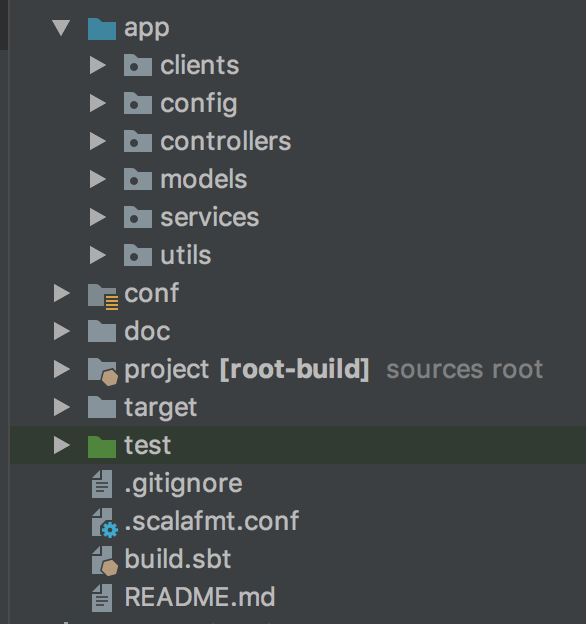
\includegraphics[width=.5\textheight]{structure}
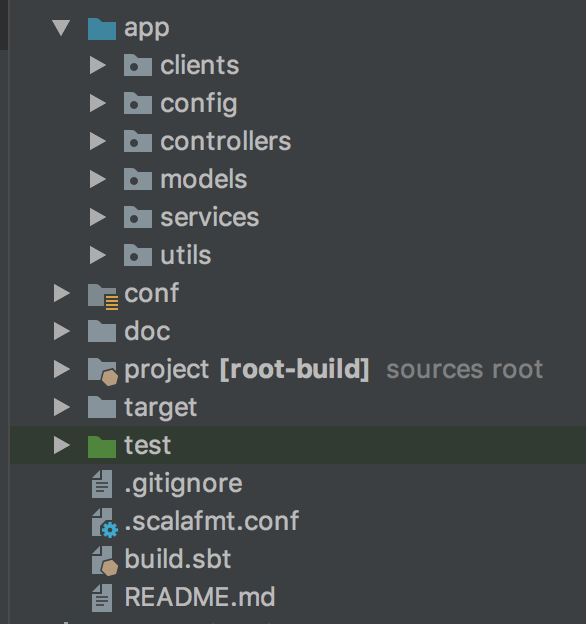
\includegraphics[height=.8\textheight]{structure}
\end{figure}
\end{frame}



%\begin{frame}
%Giter8 template 
%\end{frame}


\begin{frame}[fragile]
Routes file
\begin{lstlisting}[language=Scala, basicstyle=\ttfamily]
GET   /fetch/:id   
        controllers.Controller.fetch(id: Int)
\end{lstlisting}
\end{frame}

\begin{frame}
A taste of contract driven development:
\begin{itemize}
\item apiary / blueprint 
\item dredd testing (local / staging) 
\end{itemize}
\end{frame}

\begin{frame}
Controllers: keep them simple 
\end{frame}


\begin{frame}[fragile]
\begin{lstlisting}[language=Scala, basicstyle=\ttfamily]
@Singleton // JSR 330, guice by default 
class ProductClient @Inject()(wsClient: WSClient)  
  (implicit ex: ExecutionContext) { // implicits !! 

  def fetch() =  // using  Play wsclient 
    wsClient.url("http://test.com").get()

}
\end{lstlisting}
\end{frame}

% Error handling 
% Case classes
% Value classes
% Pattern matching 
% Option
% Future 
% implicits 



%\section{We live in a concurrent world}
%\begin{frame}[fragile]
%	% Spoiler
%	\begin{figure}
%		\centering
%		\includegraphics[width=.8\textwidth]{concurrency_coffee}
%		\caption{\url{https://joearms.github.io/published/2013-04-05-concurrent-and-parallel-programming.html}}
%	\end{figure}
%\end{frame}
%\begin{frame}[fragile]
%Is concurrency relevant for mobile development?
%	\begin{itemize} 
%		\item<2-> IO (\eg, network, etc) 
%		\item<3-> sensors (\eg, gps, etc) 
%		\item<4-> UI events 
%		\item<5-> platform lifecycle 
%	\end{itemize}
%\end{frame}

\begin{frame}
There is much more than this:
\begin{itemize}
\item Json serialization/deserialization 
\item From futures to HTTP response codes (200, non-200)
\item etc
\end{itemize}
\end{frame}

\section{Learn more}

\begin{frame}
\begin{figure}
\centering
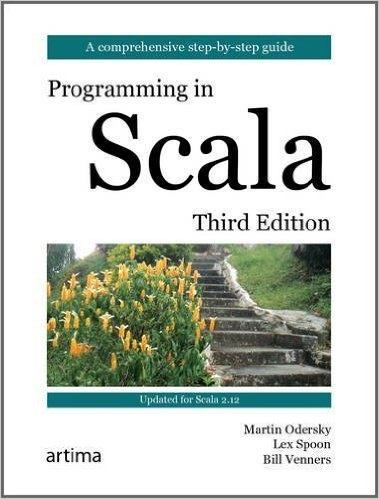
\includegraphics[height=.7\textheight]{white_book}
\caption{The reference guide}
\end{figure}
\end{frame}

\begin{frame}
\begin{figure}
\centering
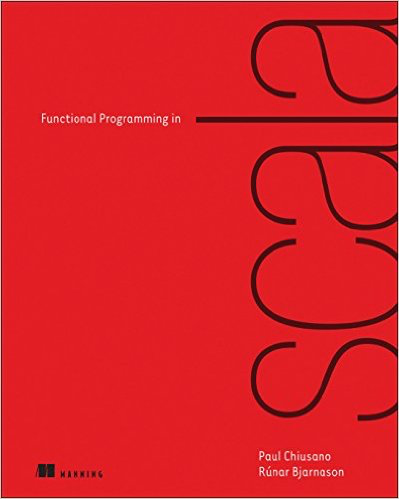
\includegraphics[height=.7\textheight]{red_book}
\caption{Gym to master FP in Scala}
\end{figure}
\end{frame}

\begin{frame}
\begin{figure}
\centering
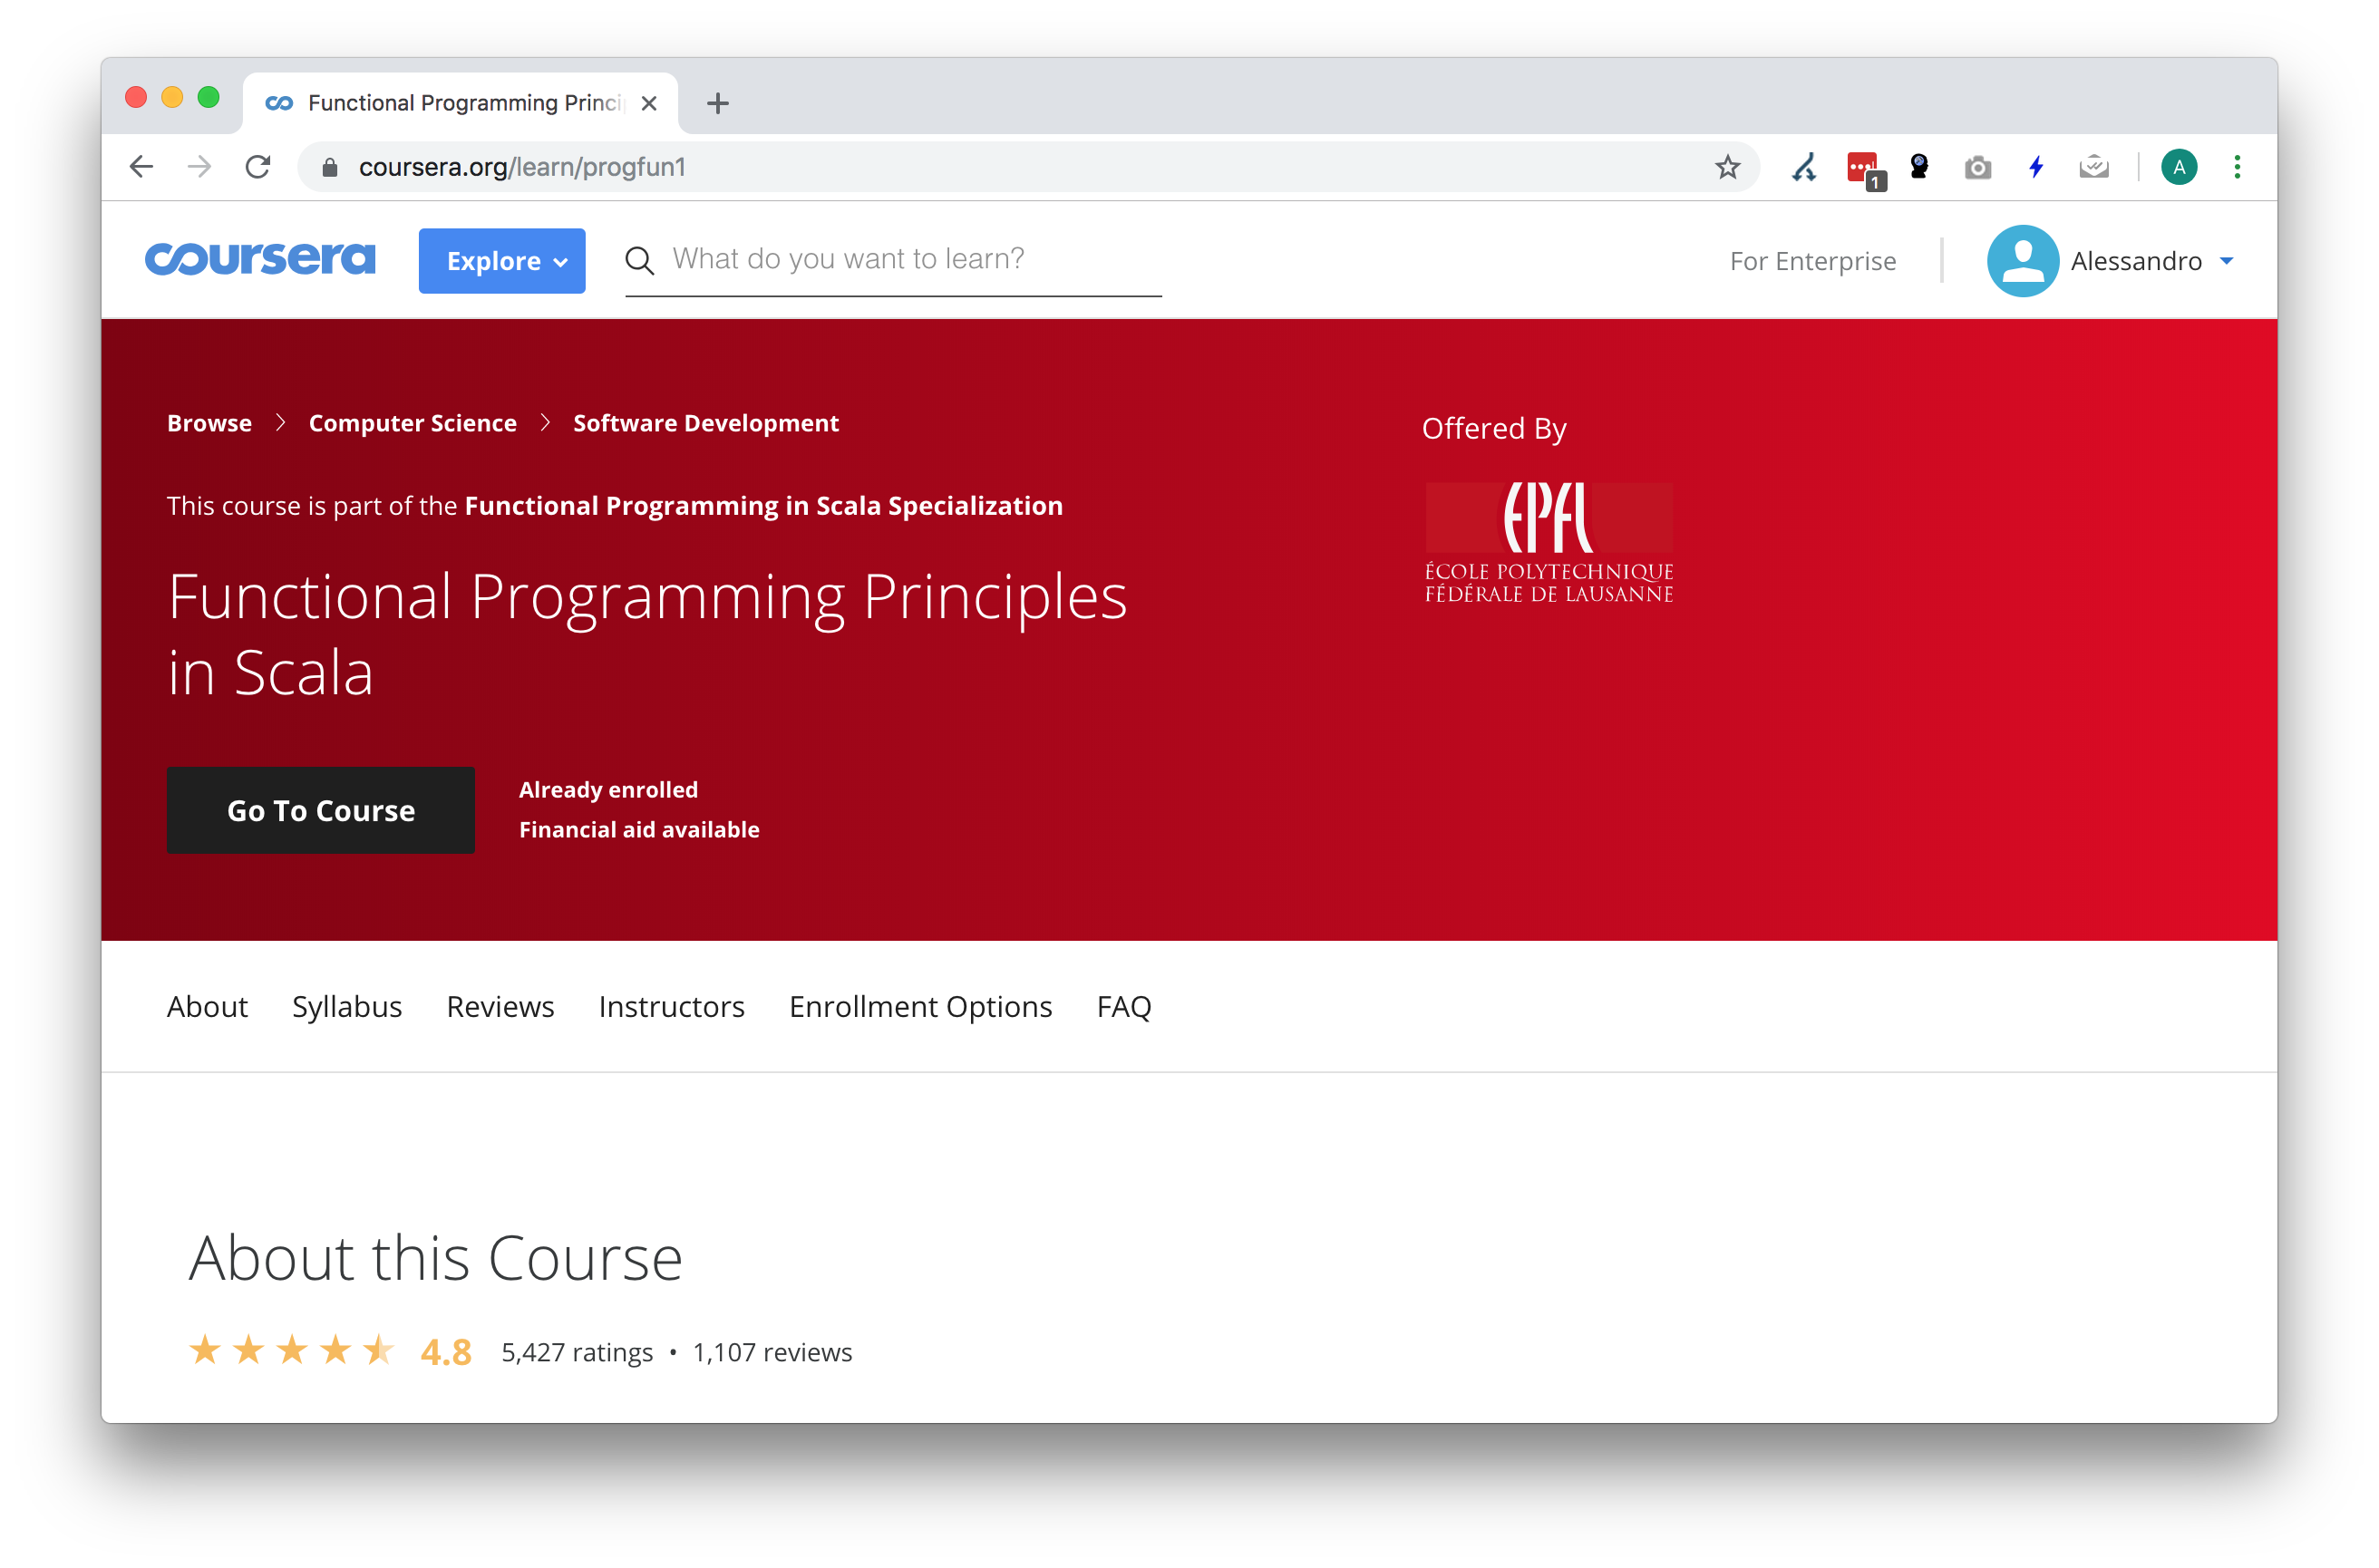
\includegraphics[width=.7\textwidth]{coursera}
\caption{Functional programming principles in Scala MOOC by Martin Odersky}
\end{figure}
\end{frame}

\begin{frame}
Online exercises:
\begin{itemize}
\item \url{https://www.scala-exercises.org/}
\item \url{http://www.scalakoans.org/}
\end{itemize}
\end{frame}

\begin{frame}[fragile]
If you are interested in FP in Scala with attention to mathematical details\ldots 


Sergei Winitzki's 
\emph{Functional programming in the mathematical spirit} video tutorials .

``Long and difficult, yet boring explanations given in excruciating detail.'' (quoting from the posts)  

First lecture here:
\begin{itemize}
\item 
\url{https://www.youtube.com/watch?v=0Ld79Lnzx_o}
\end{itemize}
\end{frame}

\plain{Questions?}

%\begin{frame}[allowframebreaks] {References}
% \bibliography{demo}
% \bibliographystyle{abbrv}
%\end{frame}

\end{document}
\begin{lstlisting}[language=Scala, basicstyle=\ttfamily]
\end{lstlisting}

\begin{frame}
\begin{lstlisting}[language=Scala, basicstyle=\ttfamily]
\end{lstlisting}
\end{frame}
